\documentclass[a4paper,12pt]{article}
\usepackage{../../mypackages}
\usepackage{../../macros}

\setlength{\parindent}{0pt}


\begin{document}

\title{Chapitre 4 : L'atome}
\author{N. Bancel}
\date{Septembre 2024}
\maketitle

\section{Introduction à l'atome}

\begin{tcolorbox}[colback=green!10!white, colframe=green!75!black, title=Définition : L'atome]
  La matière est constituée de petits grains de matière appelés atomes.
\end{tcolorbox}

Il existe plusieurs centaines d'atomes différents. Leurs noms, symboles et caractéristiques sont répertoriés dans la classification périodique des éléments. \par


\begin{figure}[H]
  \centering
  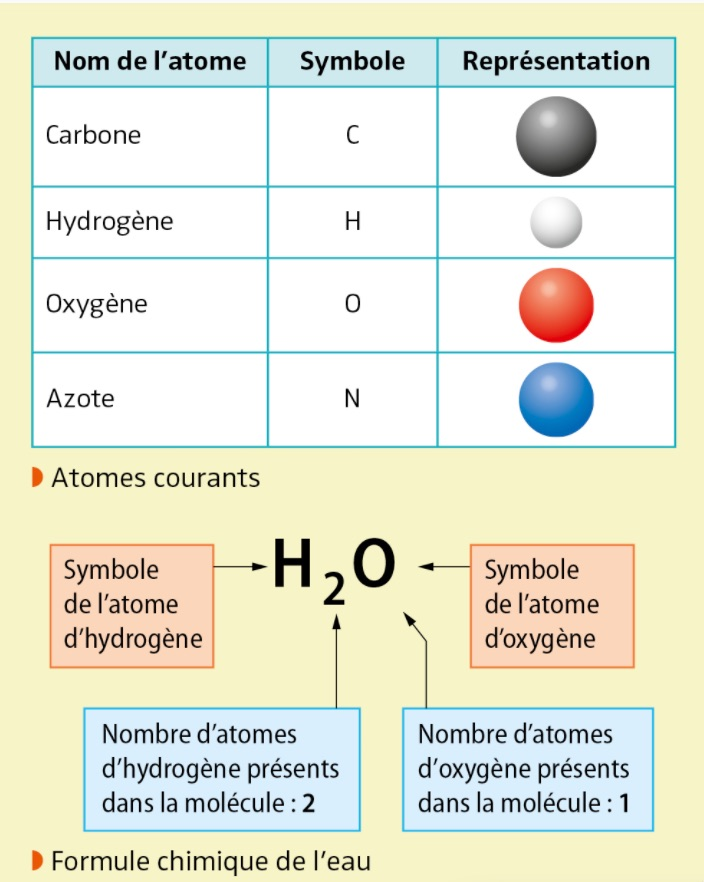
\includegraphics[width=0.3\linewidth]{atomes.jpg}
  \caption{\label{} Les principaux atomes}
\end{figure}

Leur représentation a évolué au cours du temps (Activité 10 page 35)

\begin{figure}[H]
  \centering
  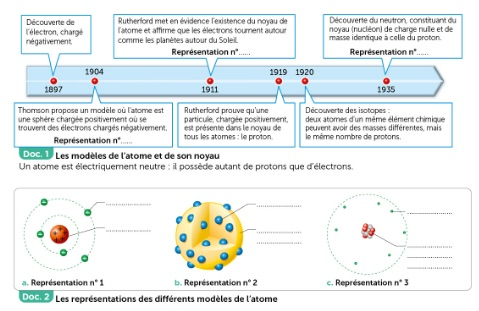
\includegraphics[width=\linewidth]{représentations_atomes.jpg}
  \caption{\label{} Les principaux atomes}
\end{figure}

\begin{enumerate}[noitemsep]
  \item 1904 : Représentation n°2
  \item 1911 - Rutherford : Représentation n°1 (protons + électrons)
  \item 1935 (influencée par la découverte des isotopes en 1920) : Deux atomes d'un même élément (donc même nombre de protons et d'électrons) peuvent avoir des masses différentes. Donc problème. Découverte en 1935 du neutron : charge nulle et masse identique à celle du proton : Représentation n°3
\end{enumerate}

\subsection{Structure de l'Atome}

\begin{tcolorbox}[colback=green!10!white, colframe=green!75!black, title=Structure de l'atome]
  Un atome est constitué d’un \textbf{noyau}, qui contient des nucléons (\textbf{protons} - Chargés positivement et \textbf{neutrons}),
et d’électrons - chargés négativement - qui gravitent autour du noyau. Le nombre de protons est appelé \textbf{numéro
atomique}, noté \textbf{Z}. Le nombre de nucléons est appelé \textbf{nombre de masse}, noté \textbf{A}. L’écriture
conventionnelle pour représenter un élément chimique est la suivante : 
\end{tcolorbox}

\begin{figure}[H]
  \centering
  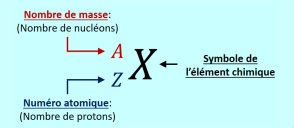
\includegraphics[width=0.3\linewidth]{symbole_atome.jpg}
  \caption{\label{} Symbole de l'atome}
\end{figure}

Puisque l'atome possède autant de protons (charges positives) que d'électrons (charges négatives), on dit que l'atome est électriquement neutre. \par 
\vspace{1em}

\[\ce{^{A \text{(nombre de masse)}}_{Z \text{(numéro atomique)}} X}\]

\[A = Z + \text{Nombre de nucléons}\] \par

Deux atomes d'un même élément ont le même nombre de protons mais peuvent avoir un nombre de neutrons différents : ce sont des isotopes 

\vspace{1em}
\textbf{Carbone 12 vs Carbone 14}

Le carbone possède 6 protons

\begin{itemize}[noitemsep]
  \item Le carbone 12 possède 12 nucléons. \ce{^{12}_{6}C} 6 neutrons
  \item Le carbone 14 possède 14 nucléons. \ce{^{14}_{6}C}. 8 neutrons
  \item Tableau périodique des éléments : 12,011 pour le carbone : parce que moyenne de toutes les masses atomiques du carbone. Plupart des atomes de carbone dans la nature sont des atomes de Carbone 12
\end{itemize}

\subsection{Dimensions de l'atome}

\subsubsection{Masse}

Masse : L'essentiel de la masse de l'atome est concentrée dans le noyau \\ 
La masse des électrons est négligeable par rapport à la masse du noyau

\vspace{1em}
\begin{tabular}{SS}
  \toprule
  {Constituant} & {Masse (en \si{kg})} \\
  \midrule
  {Electron} & {\(9.1 \times 10^{-31}\)} \\
  {Nucléon (Proton et Neutron)} & {\(1.7 \times 10^{-27}\)} \\
  \bottomrule
\end{tabular}

\vspace{1em}
\textbf{Ratio entre la masse d'un nucléon et celle d'un électron} \par 
\vspace{1em}
Le rapport entre la masse d'un nucléon et celle d'un électron peut être calculé en prenant le quotient des deux valeurs fournies dans le tableau précédent. On rappelle les valeurs des masses :
\[
m_e = 9.1 \times 10^{-31} \, \si{kg}, \quad m_n = 1.7 \times 10^{-27} \, \si{kg}
\]

Le ratio \(\frac{m_n}{m_e}\) est donc :
\[
\frac{m_n}{m_e} = \frac{1.7 \times 10^{-27}}{9.1 \times 10^{-31}}
\]

Utilisons les propriétés des puissances de 10. Lorsqu'on divise deux puissances de 10, on soustrait leurs exposants :
\[
\frac{10^{-27}}{10^{-31}} = 10^{(-27 - (-31))} = 10^{4}
\]

Le ratio des coefficients est calculé séparément :
\[
\frac{1.7}{9.1} \approx 0.187
\]

Le produit final est donc :
\[
\frac{m_n}{m_e} = 0.187 \times 10^4 = 1.87 \times 10^3
\]

Ce résultat montre que la masse d'un nucléon est environ \(1.87 \times 10^3\) fois plus grande que celle d'un électron. Cependant, pour simplifier l'ordre de grandeur, on arrondit souvent ce ratio à 2000 :
\[
\frac{m_n}{m_e} \approx 2000
\]

\paragraph{Rappel mathématique : opérations sur les puissances de 10}

Lorsque vous multipliez des puissances de 10 :
\[
10^x \times 10^y = 10^{x + y}
\]

Et lorsque vous divisez des puissances de 10 :
\[
\frac{10^x}{10^y} = 10^{x - y}
\]

Ces règles sont essentielles pour manipuler des ordres de grandeur dans des calculs scientifiques.

\subsubsection{Volume}

Volume : Occupation de l'espace : L'atome est essentiellement composé de vide. 

\vspace{1em}

\begin{tabular}{SS}
  \toprule
  {Element} & {Diamètre (en \si{m})} \\
  \midrule
  {Atome} & {\(10^{-10}\)} \\
  {Noyau} & {\(10^{-15}\)} \\
  \bottomrule
\end{tabular}


\begin{figure}[H]
  \centering
  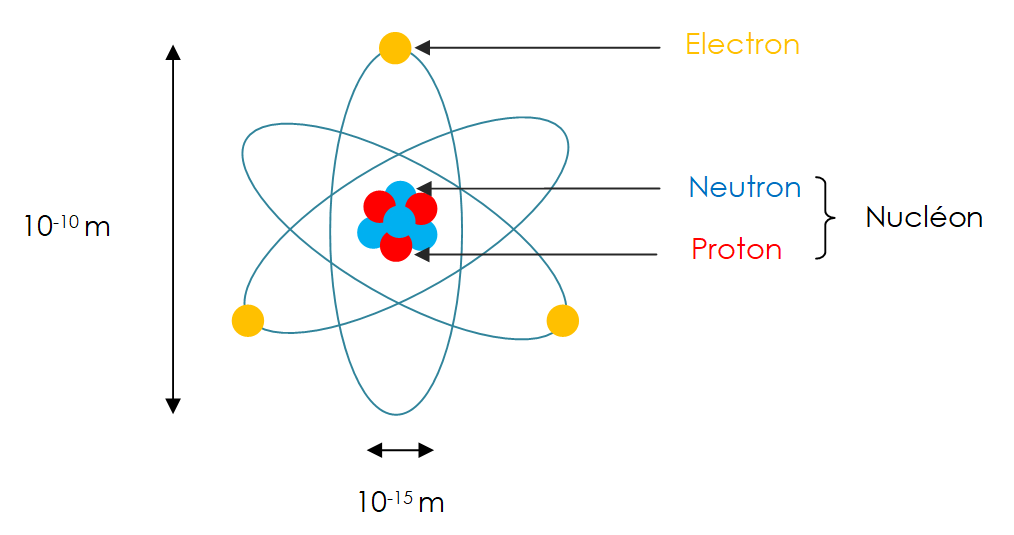
\includegraphics[width=\linewidth]{dimension_atome.png}
  \caption{\label{} Dimension de l'atome}
\end{figure}

Le noyau est 100 000 fois plus petit
Une unité a été créée pour s'adapter spécifiquement à la dimension d'un atome : le \textbf{femtomètre (symbole fm)}
Sa dimension est de \(10^{-15)}\) mètres, et correspond à la taille d'un nucléon.


\subsection{Récapitulatif de la section et devoirs à faire}

\begin{tcolorbox}[colback=blue!10!white, colframe=blue!75!black, title=Exemples - Application]
  A faire en classe 
  \begin{itemize}[noitemsep]
    \item QCM Page 39
    \item Exercice 5
    \item Exercice 6
    \item Exercice 7
    \item Exercice 8
  \end{itemize}

  A faire chez soi :
  \begin{itemize}[noitemsep]
    \item Exercice N°14 page 40
    \item Exercice N°16 page 41
  \end{itemize}
\end{tcolorbox}


\section{Les Molécules}

\begin{tcolorbox}[colback=green!10!white, colframe=green!75!black, title=Définition : Molécule]
    Une molécule est constitutée d'atomes liés entre eux
\end{tcolorbox}

La formule chimique d'une molécule indique le symbole des atomes présents dans l'ordre alphabétique et leur nombre en indice, à droite. Le chiffre 1 n'est pas indiqué.


\begin{tcolorbox}[colback=blue!10!white, colframe=blue!75!black, title=Exemples - Application]
  Quelle est la composition de chacune de ces molécules ?
  \begin{itemize}[noitemsep]
    \item Molécule de glucose : \ce{C6H12O6} 
    \item Molécule du dioxyde de carbone : \ce{CO2}
    \item Molécule d'ammoniaque : \ce{NH3} (N : azote) (entretien de maison - comme eau de Javel.)
    \item Molécule de chlorure de sodium : \ce{NaCl} (Na  : Sodium / Cl : Chlore) (Sel de table)
  \end{itemize}
\end{tcolorbox}


\section{Les réactions chimiques}

\subsection{Définitions}

\begin{tcolorbox}[colback=green!10!white, colframe=green!75!black, title=Structure de l'atome]
  Une réaction chimique est une transformation chimique au cours de laquelle les corps purs disparaissent et simultanément des corps purs nouveaux se forment (Un corps pur est composé d'une seule espèce chimique)
  Les corps purs qui disparaissent au cours d’une réaction chimique sont appelés les réactifs et les corps purs qui se forment sont appelés les produits.
\end{tcolorbox}

\begin{figure}[H]
  \centering
  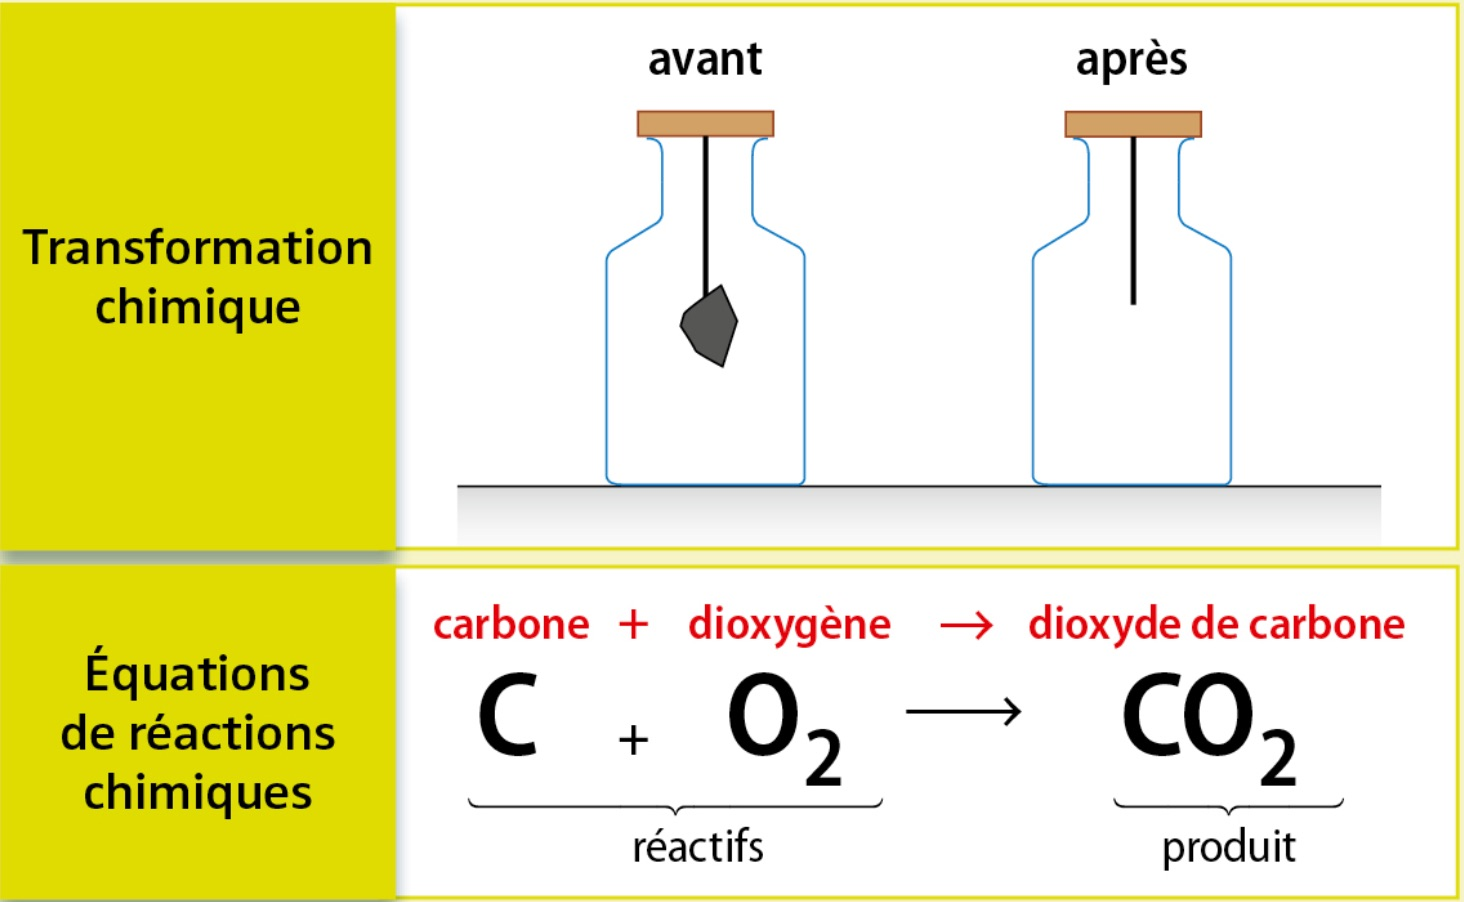
\includegraphics[width=0.5\linewidth]{equation_transformation.jpg}
  \caption{\label{} Equation x Transformation chimique}
\end{figure}

\subsection{Les équations chimiques}

\textit{Lavoisier : Rien ne se crée, rien ne se perd, tout se transforme} \par 
\vspace{1em}
Une transformation chimique est modélisée par une équation de réaction qui traduit la conservation 
\begin{itemize}[noitemsep]
  \item des éléments (\textcolor{blue}{il doit y avoir le même nombre d'atomes de part et d'autre de l'équation})
  \item des charges électriques (\textcolor{blue}{il doit y avoir le même nombre de charges de part et d'autre de l'équation})
\end{itemize}

Enjeu quand on connaît les corps purs impliqués dans une réaction chimique :

\begin{itemize}[noitemsep]
  \item connaître le \# d'atomes qui réagissent entre eux, pour garantir qu'on conserve bien la charge, et la masse.
  \item On dit qu'on cherche à \textbf{équilibrer} l'équation.
\end{itemize} \par

Autrement dit, équilibrer une équation revient à déterminer les proportions dans lesquelles les réactifs réagissent et les produits se forment. \par

\begin{itemize}[noitemsep]
  \item Il est interdit de toucher aux formules des molécules : on cherche les coefficients par lesquels il faut multiplier les molécules pour équilibrer l'équation.
  \item Ces coefficients sont appelés les coefficients stoechiométriques
\end{itemize}

\begin{figure}[H]
  \centering
  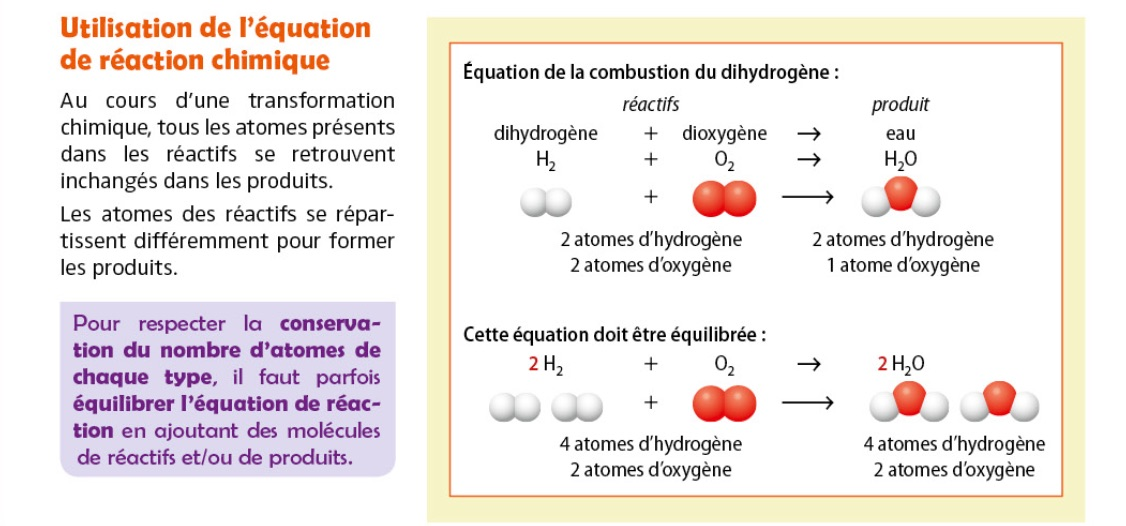
\includegraphics[width=0.9\linewidth]{reaction_chimique.jpg}
  \caption{\label{} Réaction Chimique}
\end{figure}

\begin{tcolorbox}[colback=blue!10!white, colframe=blue!75!black, title=Exemples - Application]
  Combustion du méthane dans le dioxygène. L'équation du dessous est-elle équilibrée ?
  \begin{figure}[H]
    \centering
    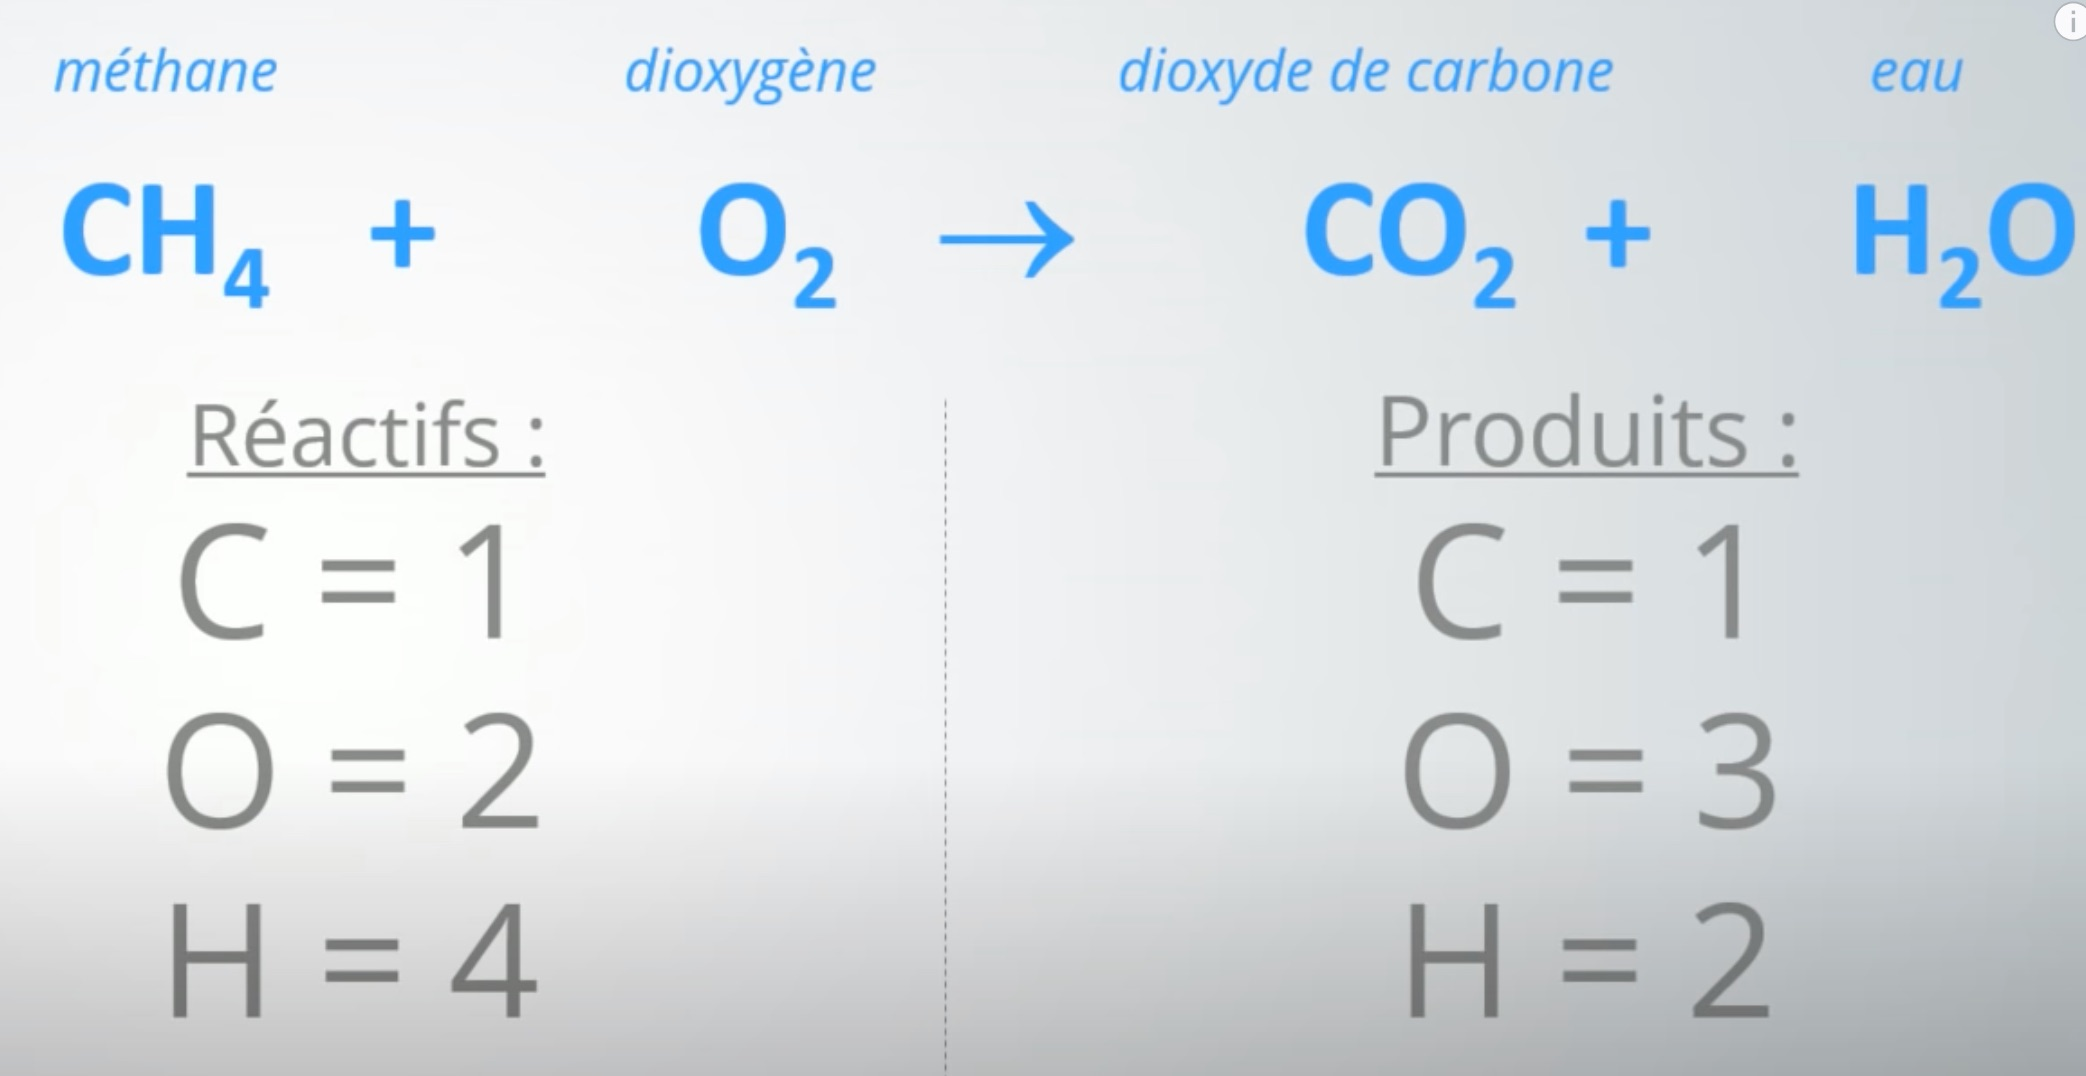
\includegraphics[width=0.5\linewidth]{equation_methane.jpg}
    \caption{\label{} Combusion du méthane}
  \end{figure}

  Source : \href{https://www.youtube.com/watch?v=VZVBS4OwwlE&ab_channel=PaulOlivier}{Paul Olivier - Comment équilibrer une équation chimique ? (Physique-Chimie)} \par
  \vspace{1em}
  
  Le dioxyde de carbone se dissout dans l'eau lors d'une transformation chimique. \par
  Quelle équation chimique représente cette dissolution ?

  \begin{enumerate}[noitemsep]
    \item \ce{CO2 + H2O -> 2 H+ + CO_3^{2-}}
    \item \ce{2 H+ + CO_3^{2-} -> CO2 + H2O}
    \item \ce{CO2 + H2O -> H+ + CO_3^{2-}}
  \end{enumerate}

  Source : \href{https://www.youtube.com/watch?v=KRimPPjL9xg&ab_channel=PaulOlivier}{Paul Olivier - Équilibrer équation chimique, difficile } \par

  \textbf{Exemples bonus} : quelques équations chimiques supplémentaires

  \begin{enumerate}[noitemsep]
    \item \ce{C6H12O6 -> 2 C2H5OH + 2 CO2} (Fermentation du glucose pour former l'éthanol et du dioxyde de carbone)
    \item \ce{2 Fe + 3 Cl2 -> 2 FeCl3}
  \end{enumerate}

\end{tcolorbox}

\subsection{La conservation de la masse}

\begin{figure}[H]
  \centering
  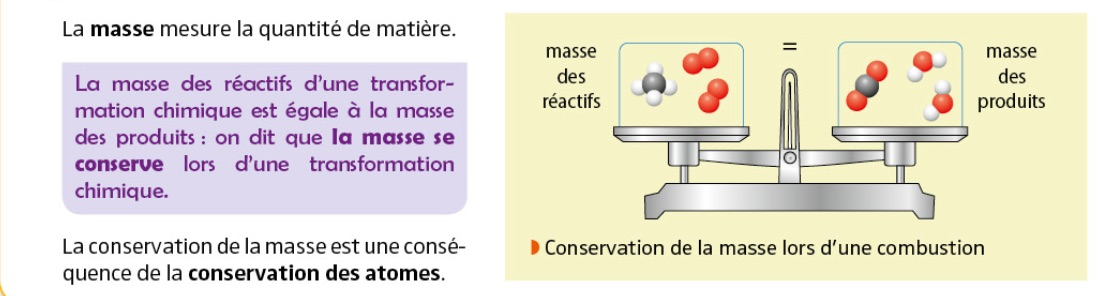
\includegraphics[width=0.5\linewidth]{conservation_masse.jpg}
  \caption{\label{} Conservation de la masse}
\end{figure}

\section{Articles / vidéos intéressants}

\begin{enumerate}[noitemsep]
  \item \href{https://www.superprof.fr/ressources/physique-chimie/physique-chimie-tous-niveaux/formule-chimique-scientifique.html}{Quelques molécules importantes}
  \item xxxx
\end{enumerate}


\end{document}
